\documentclass[a4paper, 11pt]{article}
\usepackage{comment} % enables the use of multi-line comments (\ifx \fi) 
\usepackage{fullpage} % changes the margin
\usepackage{hyperref}
\usepackage{mathtools}
\usepackage{amsmath}
\usepackage{amssymb}
\usepackage{longtable}
\usepackage{booktabs} % For formal tables
\usepackage[ruled]{algorithm2e} % For algorithms
\renewcommand{\algorithmcfname}{ALGORITHM}
\DeclarePairedDelimiter{\ceil}{\lceil}{\rceil}

\begin{document}

\begin{titlepage}
   \begin{center}
       \vspace*{1cm}
 
       \textbf{\huge{SOEN 6011: SOFTWARE ENGINEERING PROCESSES}}
 
       \vspace{0.5cm}
        \textbf{\huge{Project Deliverable 2}}
 
       \vspace{1.0cm}
       \vskip 1.4in
    
\includegraphics[width=1.0\textwidth]{Concordia.jpg}
       
       \vskip 1.4in
 
       \vspace{0.8cm}
       \textbf{GitHub Repository : \url{https://github.com/Hkohli30/SOEN_6011}}\\
       
        \textbf{Himanshu Kohli}\\
        \textbf{Student Id : 40070839}\\
       Applied Computer Science\\
       Concordia University\\
       
 
   \end{center}
\end{titlepage}

% @author : Himanshu Kohli
% Student ID: 40070839
% Date: 29 July 2019
\noindent
\large\textbf{Problem 4 and 6} \hfill \textbf{Himanshu Kohli} \\
\normalsize SOEN 6011 \hfill \textbf{40070839} \\
Prof. Pankaj Kamthan \hfill Due Date: July 29, 2019 \\


\section{Debugger}
\subsection{Introduction}
Debugging is a process of locating and removing bugs, errors and abnormalities form a programs. Bugs are subtle conditions which leads inefficient programs and can only be found when specific conditions occurs.
\subsection{Debugger Used}
The Eclipse IDE provides a bug finding tool which is combined in the views as Debug perspective which helps us to view execution of the program and the variables/constant at every stage of the program. Eclipse IDE Debugger is an source-level debugger or symbolic debugger which finds traps(conditions which doesn't allow the program to execute normally) in the system. Eclipse inbuilt debgger has many features which helps such as:\cite{wikipedaDebugger} \cite{eclipse}
\begin{enumerate}
    \item Single Stepping : A step by step execution of program helps the programmer understand, see and find the error by viewing the values of all the variables.
    \item Breakpoints: Pausing the state of the program for examination 
    \item Tracepoints : Allows user to create conditional breakpoints to print messages without halting the breakpoints
\end{enumerate}
\subsection{Advantages and Disadvantages}
\subsubsection{Advantages}
\begin{enumerate}
    \item \textbf{Watches} in debugging eliminates the need to add additional print line statements to the source code and removing it after finding the bug.
    \item It removes the tedious and time consuming process of rebuilding and executing the program while at most times \textbf{hot swapping} the changes.
    \item Stepping in and out of some part of the code saves time for the user and increase programmer's efficiency to find bugs.
\end{enumerate}

\subsubsection{Disadvantages}
\begin{enumerate}
    \item For a smaller code which can be understood by print line statement it can be rather time consuming to use debugger
    \item Overloads the system's resources in getting value of all variables at execution time.
\end{enumerate}


\newpage
\section{Code Quality Checking Tool }
\subsection{Introduction}
Code quality checking technically known as Static program analysis tool which is the analysis of the computer program without the actual execution of program. These software may vary and might target source code or the object code of the program. They have rules defined in their definition of the program and compare the source code with their definition and notify user of the modification which will make the program more feasible.\cite{wikiStatic}
\subsection{Tool Used}
PMD is an open source static source code analyzer that reports the issues found within the application. It compares the source with set of build in rules and report issues. Custom rules also can be defined by the user to handle specific issues or apply constrains. The issues reported are inefficient code or bad programming habits which reduces the maintainability and efficiency of the program. \cite{wikiPMD}
\subsection{Advantages and Disadvantages}
\subsubsection{Advantages}
\begin{enumerate}
    \item Possibility of finding bugs using tool.
    \item Removes redundancy in the application such as removing unwanted loops or code.
    \item Sub optimal code : avoids the usage of strings and string buffer which takes memory but do not utilize it. 
    \item Dead Code : Reports the usage of code which is declared but not used in the program.
    \item Reports over complicated errors such as replacing 'if' statement with loops.
\end{enumerate}
\subsubsection{Disadvantages}
\begin{enumerate}
    \item Sometimes report normal coding as error such as indentation errors or Java Docs needed errors
    \item Does not support chain programming
    \item Global variable declaration error.
    \item Errors in normal access specifiers such as if the default access specifier is public and you specify public for a method, it will result in error.
\end{enumerate}

\newpage
\subsection{Quality Attributes}
The implemented program for function $a^{b^x}$ aims to achieve all the following quality attributes and all the necessary steps taken to make the program more tenacious.
\subsubsection{Correct}
The program aims the results to be correct and handles larger and smaller values. The program implements log function and power function from scratch aiming to achieve actual calculator results. So two forms of power function were implemented one for decimal and one for integers for the exponent in order to achieve correct results. JUnit test cases for each and every value were tested and generated like-wise results for the values. 
\subsubsection{Efficient}
The program implemented is efficient and only calculate values until it reaches the max value for double specifies it as positive or negative infinity, nullifying extra calculations whose results cannot be printed, saving computation time of the program. The bounding conditions are handled properly so that the function doesn't have to perform extra calculation and increase the efficiency in providing results.  Try catch block maintains the state of the program while execution without having the program to be restarted making it efficient.
\subsubsection{Maintainable}
The program's implementation of Memento design pattern help the program memorize it's last result and make the program able to recall the result without any additional storage data structure. With using design patterns the program maintainability increases as everything divides into set of modules each pertaining to its own functionality which is easier to track, understand and modify. And the implementation of try catch helps the program.
\subsubsection{Robust}
The implementation of try catch block not only saves time but act as an shield to the erroneous inputs by the user such as a complex number or alphabetic values to the program. The program uses Taylor series to execute and converts $b^x$ to $e^{x * \log b}$ where there are no values for $\log \leq 0$. And the program handles it without crashing making it secure and efficient.
\subsubsection{Usability}
The implementation of the Memento design pattern has divided the programming into modules which can be used for multiple other implementation of the program by just the main logic of the program. Even the logic part of the program is divided into modules which helps aim usability/re-usability of the program.

\newpage
\subsection{Traceability and Coverage}
\subsubsection{Test Case Traceability}

\begin{center}
\begin{longtable}{|l|l|l|}
\caption{Test case traceability table.} \label{tab:long} \\

\hline \multicolumn{1}{|c|}{\textbf{Test Case #}} & \multicolumn{1}{c|}{\textbf{Test Case Name}} & \multicolumn{1}{c|}{\textbf{Related Requirement(s)}} \\ \hline 
\endfirsthead

\multicolumn{3}{c}%
{{\bfseries \tablename\ \thetable{} -- continued from previous page}} \\
\hline \multicolumn{1}{|c|}{\textbf{Test Case #}} & \multicolumn{1}{c|}{\textbf{Test Case Name}} & \multicolumn{1}{c|}{\textbf{Related Requirement(s)}} \\ \hline 
\endhead

\hline \multicolumn{3}{|r|}{{Continued on next page}} \\ \hline
\endfoot

\hline \hline
\endlastfoot

1 & testForPowerFunctionIntegerValues() & FRQ3 \\
2 & testForLogValue() & FRQ1, FRQ2 \\
3 & testForPowerFunctionLargeValues() & FRQ4, FRQ5 \\
4 & testForPowerFunctionDecimalValues()  & FRQ3 \\
5 & testForEntireFunction() & FRQ8, FRQ7,FRQ6 \\
6 & signTestingForPowerFunction() & FRQ8 \\
7 & inputTestingForValidInputs() & FRQ1, FRQ3 \\
8 & inputTestingForInvalidInputs() & FRQ1, FRQ3 \\
\end{longtable}
\end{center}

\subsubsection{Code Coverage}

\begin{figure}[h]
\caption{Representation of the code coverage for random inputs}
\centering
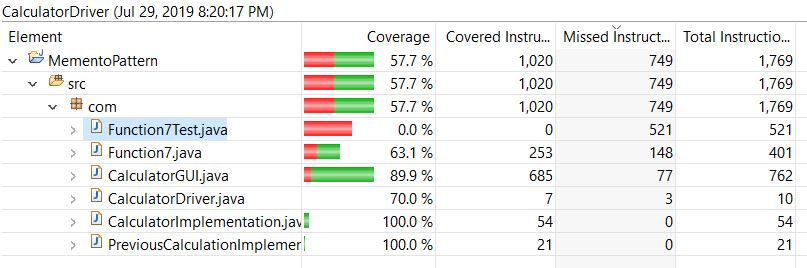
\includegraphics[width=0.7\textwidth]{coverage.JPG}
\end{figure}

\subsubsection{Execution Screen Shot}

\begin{figure}[h]
\caption{Representation of the main screen}
\centering
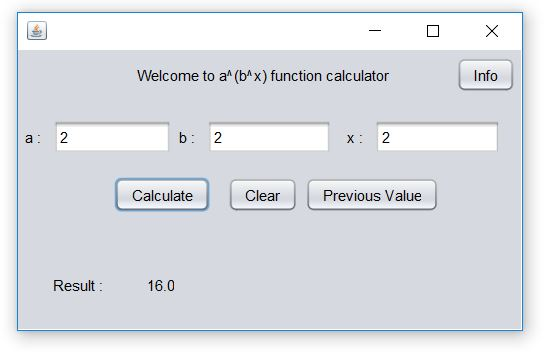
\includegraphics[width=0.59\textwidth]{screenshot.JPG}
\end{figure}

\newpage
\begin{thebibliography}{}
\bibitem{wikipedaDebugger} 
Debugger
\url{https://en.wikipedia.org/wiki/Debugger}
\bibitem{eclipse}
Debugging the Eclipse IDE for Java Developers | The Eclipse Foundation
\url{https://www.eclipse.org/community/eclipse_newsletter/2017/june/article1.php}
\bibitem{stackDebug}
What are the advantages of using the Java debugger over println?
\url{https://softwareengineering.stackexchange.com/questions/168540/what-are-the-advantages-of-using-}
\bibitem{wikiStatic}
Static program analysis
\url{https://en.wikipedia.org/wiki/Static_program_analysis}
\bibitem{wikiPMD}
PMD (software)
\url{https://en.wikipedia.org/wiki/PMD_(software)}
\bibitem{wikiQuality}
List of system quality attributes
\url{https://en.wikipedia.org/wiki/List_of_system_quality_attributes}

\end{thebibliography}

\end{document}